\documentclass[runningheads]{llncs}
\usepackage[T1]{fontenc}
\usepackage{amsmath,amssymb,booktabs,graphicx}
\usepackage[hidelinks]{hyperref}
\hypersetup{pdfauthor={Shayan Bemanian}}
\newcommand{\PublicationResultsRows}{%
LightGCN & $0.1386\pm0.0012$ & $0.0849\pm0.0004$ & $0.1130\pm0.0026$ & $0.0713\pm0.0017$ & $0.1319\pm0.0007$ & $0.0834\pm0.0005$ \\
Full RLMRec & $0.1465\pm0.0023$ & $0.0894\pm0.0010$ & $0.1227\pm0.0015$ & $0.0769\pm0.0010$ & $0.1424\pm0.0009$ & $0.0903\pm0.0005$ \\
Item-only RLMRec & $0.1462\pm0.0013$ & $0.0895\pm0.0006$ & $0.1225\pm0.0016$ & $0.0773\pm0.0005$ & $0.1410\pm0.0006$ & $0.0893\pm0.0002$ \\
SIG & $0.1536\pm0.0016$ & $0.0935\pm0.0007$ & $0.1199\pm0.0010$ & $0.0757\pm0.0006$ & $0.1471\pm0.0002$ & $0.0931\pm0.0002$ \\
}

\newcommand{\PublicationEffectRows}{%
Amazon & SIG $-$ full RLMRec & $+0.00705$ & $[+0.00295, +0.01115]$ & 0.0088 & 0.0354 & 0.0625 \\
Amazon & Item-only $-$ full RLMRec & $-0.00027$ & $[-0.00182, +0.00129]$ & 0.6604 & 1.0000 & 0.6875 \\
Yelp & SIG $-$ full RLMRec & $-0.00281$ & $[-0.00400, -0.00162]$ & 0.0028 & 0.0197 & 0.0625 \\
Yelp & Item-only $-$ full RLMRec & $-0.00015$ & $[-0.00255, +0.00224]$ & 0.8693 & 1.0000 & 0.7500 \\
Steam & SIG $-$ full RLMRec & $+0.00474$ & $[+0.00376, +0.00572]$ & 0.0002 & 0.0017 & 0.0625 \\
Steam & Item-only $-$ full RLMRec & $-0.00139$ & $[-0.00231, -0.00047]$ & 0.0140 & 0.0419 & 0.0625 \\
}

\newcommand{\PublicationSensitivityRows}{%
Amazon & 0.003 & 0.15020 & 0.14836 & $-0.00184$ \\
Amazon & 0.01 & 0.14984 & 0.15004 & $+0.00020$ \\
Amazon & 0.03 & 0.14378 & 0.14737 & $+0.00359$ \\
Yelp & 0.003 & 0.12379 & 0.12379 & $+0.00000$ \\
Yelp & 0.01 & 0.12407 & 0.12442 & $+0.00035$ \\
Yelp & 0.03 & 0.03805 & 0.11889 & $+0.08085$ \\
}

\newcommand{\PublicationFocusedMainRows}{%
Amazon & LightGCN & $0.1386\pm0.0012$ & $0.0849\pm0.0004$ \\
Amazon & Full RLMRec & $0.1465\pm0.0023$ & $0.0894\pm0.0010$ \\
Amazon & Item-only RLMRec & $0.1462\pm0.0013$ & $0.0895\pm0.0006$ \\
Yelp & LightGCN & $0.1130\pm0.0026$ & $0.0713\pm0.0017$ \\
Yelp & Full RLMRec & $0.1227\pm0.0015$ & $0.0769\pm0.0010$ \\
Yelp & Item-only RLMRec & $0.1225\pm0.0016$ & $0.0773\pm0.0005$ \\
Steam & LightGCN & $0.1319\pm0.0007$ & $0.0834\pm0.0005$ \\
Steam & Full RLMRec & $0.1424\pm0.0009$ & $0.0903\pm0.0005$ \\
Steam & Item-only RLMRec & $0.1410\pm0.0006$ & $0.0893\pm0.0002$ \\
}

\newcommand{\PublicationFocusedEffectRows}{%
Amazon & $-0.00027$ & $[-0.00182, +0.00129]$ & 1.0000 & 0.6875 \\
Yelp & $-0.00015$ & $[-0.00255, +0.00224]$ & 1.0000 & 0.7500 \\
Steam & $-0.00139$ & $[-0.00231, -0.00047]$ & 0.0419 & 0.0625 \\
}

\newcommand{\PublicationPatienceRows}{%
2023 & 0.11587 & 0.11866 & 84 & 66 \\
2025 & 0.11605 & 0.11991 & 72 & 63 \\
}

\newcommand{\PublicationPublishedRows}{%
Amazon & LightGCN & 0.1411 & 0.1403 & $-0.0008$ & 0.0856 & 0.0856 & $+0.0000$ \\
Amazon & RLMRec-Con & 0.1483 & 0.1477 & $-0.0006$ & 0.0903 & 0.0900 & $-0.0003$ \\
Yelp & LightGCN & 0.1157 & 0.1130 & $-0.0027$ & 0.0733 & 0.0713 & $-0.0020$ \\
Yelp & RLMRec-Con & 0.1230 & 0.1227 & $-0.0003$ & 0.0776 & 0.0769 & $-0.0007$ \\
Steam & LightGCN & 0.1348 & 0.1319 & $-0.0029$ & 0.0855 & 0.0834 & $-0.0021$ \\
Steam & RLMRec-Con & 0.1421 & 0.1424 & $+0.0003$ & 0.0902 & 0.0903 & $+0.0001$ \\
}

\newcommand{\PublicationProtocolRows}{%
32 & 4096 & 0.1477 & 0.1482 & $+0.00051$ & $[-0.00209, +0.00310]$ & $+0.00030$ & 0.636 \\
32 & 1024 & 0.1465 & 0.1462 & $-0.00027$ & $[-0.00182, +0.00129]$ & $+0.00002$ & 0.945 \\
64 & 1024 & 0.1569 & 0.1569 & $-0.00001$ & $[-0.00099, +0.00098]$ & $+0.00045$ & 0.046 \\
}

\title{Revisiting RLMRec: User-Profile Alignment, Early Stopping, and Reproducibility}
\titlerunning{Revisiting RLMRec}
\author{Shayan Bemanian}
\authorrunning{Shayan Bemanian}
\institute{}
\begin{document}
\maketitle

\begin{abstract}
RLMRec improves a graph recommender by pulling its user and item embeddings
toward text profiles written by a large language model. Writing a profile for
every user is expensive, so we ask a simple question: are the user profiles
worth it? We rerun the released RLMRec code on its three benchmark datasets,
then remove only the part of the training objective that uses user profiles.
The released code reproduces the published results closely. Without user
profiles, we could not detect any change on Amazon-book or Yelp, but on Steam
the model loses a small amount of accuracy, consistently across every seed.
Along the way, we found that a dramatic failure of the full model on Yelp was
not real: training stalls for a while, and the usual early-stopping rule gives
up just before it recovers. Whether user profiles help therefore depends on
the dataset, and ablation results should be read alongside training curves,
not just final scores.

\keywords{Recommendation \and Language models \and Reproducibility \and Ablation studies}
\end{abstract}

\section{Introduction}
RLMRec~\cite{rlmrec} uses a large language model (LLM) to write a short text
profile for every user and every item, turns those profiles into embeddings,
and trains a recommender so that its own embeddings line up with them. Item
profiles and user profiles are not equally cheap: every user needs their own
LLM call. This makes a practical question worth asking: once item profiles are
in place, do user profiles add any accuracy?

The original paper does not answer this directly. Its ablation (Section 4.3
of~\cite{rlmrec}) shuffles the semantic representations and swaps the text
encoder. That tells us whether matching the right profile to the right user or
item matters. It does not tell us how much each part of the objective
contributes on its own. To measure that, we keep everything else fixed,
including the released embeddings, and delete one term: the loss that aligns
users with their profiles.

We work with the released LightGCN version of RLMRec-Con and ask four
questions:
\begin{description}
\item[RQ1] Does the released code reproduce the published results?
\item[RQ2] How much does aligning users with their profiles add on top of
aligning items?
\item[RQ3] Why does the full model seem to break on Yelp when the alignment
weight is high?
\item[RQ4] How much do repeated runs with the same seed differ on our hardware?
\end{description}
In short: the published RLMRec-Con results reproduce well on all three
datasets. User profiles help a little on Steam, and we could not detect any
benefit on Amazon or Yelp. One large effect we saw along the way turned out to
be caused by stopping training too early, and the training curves make this
easy to spot. This is a reproduction and ablation study; we do not propose a
new model.

\section{Background and Compared Objectives}
LightGCN~\cite{lightgcn} learns an ID embedding for each user and item and
smooths these embeddings over the user--item interaction graph.
RLMRec~\cite{rlmrec} adds a second signal: it aligns these embeddings with
LLM-generated profiles, either contrastively (Con) or generatively (Gen).
Other work uses LLMs in different ways. LLMRec~\cite{llmrec} adds
LLM-generated edges and attributes to the interaction graph.
AlphaRec~\cite{alpharec} shows that language representations of items alone
can support strong recommendation, and also tries alternative inputs for
RLMRec. Our approach is narrower: we keep RLMRec's released inputs exactly as
they are and remove a single alignment term.

Two lessons from earlier reproducibility work shape how we read our results.
Gains reported for neural recommenders often shrink once the baselines are
tuned properly~\cite{dacrema,rendle-baselines}, and the variation from one
run to the next can be as large as the improvement being
claimed~\cite{bouthillier}. Ablation studies are exposed to both problems.

\paragraph{The ranking loss.}
Each training batch holds $B$ triples $(u,i,j)$: user $u$ interacted with item
$i$, and item $j$ is sampled from outside $u$'s training history. The model
gives each user--item pair a score $\hat y_{ui}=h_u^\top h_i$, where $h$ are
the collaborative embeddings. The BPR loss~\cite{bpr} rewards the model for
scoring $i$ above $j$:
\begin{equation}
 \overline{\mathcal L}_{\rm BPR}=\frac{1}{B}\sum_{(u,i,j)}
 \operatorname{softplus}(\hat y_{uj}-\hat y_{ui}).
\end{equation}
When the model cannot tell positive items from negative ones, this loss equals
exactly $\ln 2$. This value becomes important in Section~\ref{sec:stopping}.

\paragraph{The alignment losses.}
Each profile is represented by a frozen 1536-dimensional semantic vector. A
small shared network $g$ (a two-layer MLP) projects these vectors down to the
size of the collaborative embeddings. Three contrastive InfoNCE
losses~\cite{infonce} then pull each embedding toward its own projected
profile and away from the others: $\overline{\mathcal L}_u$ for users,
$\overline{\mathcal L}_{i^+}$ for positive items, and
$\overline{\mathcal L}_{i^-}$ for negative items, each averaged over the batch
and using cosine similarity. As in the released code, each user is compared
against all projected user profiles, while each item loss compares against the
items in the current batch, keeping repeated items. The full objective and our
item-only variant are
\begin{align}
 \mathcal L_{\rm full}&=\overline{\mathcal L}_{\rm BPR}
 +\alpha(\overline{\mathcal L}_u+\overline{\mathcal L}_{i^+}
 +\overline{\mathcal L}_{i^-})+\beta\|\Theta\|_2^2,\\
 \mathcal L_{\rm item}&=\overline{\mathcal L}_{\rm BPR}
 +\alpha(\overline{\mathcal L}_{i^+}+\overline{\mathcal L}_{i^-})
 +\beta\|\Theta\|_2^2.
\end{align}
The only change is that $\overline{\mathcal L}_u$ is gone; every coefficient
stays the same. This has two side effects to keep in mind. The total weight
on alignment becomes smaller, and the shared projector $g$ no longer learns
anything from user profiles. Our comparison therefore measures ``remove the
user term'', not ``same total alignment, but without users''. Both variants
keep the released code's other choices: summing the outputs of layers 0--3,
dropping edges without rescaling the ones that remain, and squared-norm
regularization of all parameters.

\section{Reproduction Setup}
\paragraph{Implementation.}
We rebuilt the training code from the released RLMRec repository; the
artifact records the full hash of commit \texttt{22413752246d}. Four details
of that code decide what is actually being optimized, so we matched them
exactly: summing the layer outputs, edge dropout without rescaling, squared
regularization of all parameters, and separate candidate sets for the user and
item contrastive losses. Some of our earlier LightGCN implementations differed
in the readout or the regularization, and we excluded them. Two models can
share a name and still optimize different objectives.

We made one deliberate fix. The code caches embeddings, and we clear this
cache before every evaluation and after restoring a checkpoint, so evaluation
always uses embeddings computed from the current weights. Unit and integration
tests cover the objective, how the model is wired together, the graph
operations and the cache. All training runs on Apple's MPS GPU backend, with
sparse graph propagation implemented through gather and scatter operations.

\paragraph{Data.}
\begin{table}[t]
\caption{Dataset sizes. Interaction counts are for the training, validation
and test splits.}
\label{tab:data}\centering\small
\begin{tabular}{lrrrrr}
\toprule
Dataset & Users & Items & Train & Validation & Test\\\midrule
Amazon-book & 11,000 & 9,332 & 120,464 & 40,290 & 40,106\\
Yelp & 11,091 & 11,010 & 166,620 & 55,479 & 55,436\\
Steam & 23,310 & 5,237 & 316,190 & 104,897 & 104,835\\
\bottomrule\end{tabular}
\end{table}
We use RLMRec's released interaction data and semantic embeddings and do not
regenerate any profiles. Table~\ref{tab:data} summarizes the three datasets.
We checked that the training, validation and test splits share no user--item
pairs, and that the semantic inputs have the expected shapes and contain only
finite values. The interaction graph is built from training data only. At
evaluation time, each user's candidates are all items except those in their
training data; validation items stay in the candidate list during testing.
Recall and NDCG are averaged over the users who have at least one positive
item in the split being evaluated.

\paragraph{Training and model selection.}
All models use 32-dimensional embeddings, three graph layers, and Adam with a
learning rate of $10^{-3}$ and no weight decay in the optimizer. Both RLMRec
variants use alignment weight $\alpha=0.01$, temperature $0.2$, an edge keep
rate of $0.8$ and regularization weight $\beta=10^{-7}$. On Yelp and Steam we
use the published batch size of 4096. Our main Amazon comparison uses 1024,
and Section~\ref{sec:rq2} repeats it at 4096.

Every three epochs we compute Recall@20 on the validation set. When training
ends, we restore the best checkpoint and evaluate it on the test set exactly
once. Training stops after five evaluations without improvement on Amazon and
Yelp, and after 25 on Steam. The longer Steam patience was added later, and
Section~\ref{sec:rq2} shows that it does not change which checkpoints are
chosen. Every comparison uses the same five seeds: 1, 7, 13, 42 and 2024. All
45 main runs stopped early, and none picked a checkpoint from before epoch 24.

\paragraph{Statistics.}
All comparisons are paired by seed. We report sample standard deviations, 95\%
paired Student-$t$ confidence intervals, paired $t$-tests, and exact two-sided
sign-flip tests. With only five pairs, the sign-flip test can never give a
$p$-value below $0.0625$, even when every pair points the same way.

We correct for multiple comparisons with Holm's method~\cite{holm}, over
twelve contrasts per metric. On each dataset these are: full and item-only
RLMRec versus LightGCN, item-only versus full, and an archived graph recipe in
the style of FREEDOM~\cite{freedom} versus full. The graph-recipe results
appear only in the artifact. Leaving them out of the correction changes none
of our conclusions, and the Steam item-only contrast keeps its adjusted
$p=0.042$. The confidence intervals are not adjusted for multiple comparisons.

Two cautions apply throughout. We did not fix an equivalence margin in
advance, so a non-significant difference means ``not detected'', not ``the
same''. And the study is retrospective: we had already seen development and
test results when we decided how to frame it.

\paragraph{Diagnostic runs.}
Three smaller sets of runs support the main comparison. None of them is
pooled with the five-seed results or used to choose settings. First, a
validation-only grid runs both RLMRec variants at $\alpha=0.003$, $0.01$ and
$0.03$ on Amazon and Yelp, with development seed 2023. Second, because the
full model failed at Yelp $\alpha=0.03$ in that grid, we reran that setting
with patience 20 on seeds 2023 and 2025 (four runs, again validation only).
Third, to see how repeatable a single seed is, we ran each variant four times
on Amazon at $\alpha=0.01$ with seed 42.

\section{Results}
\subsection{RQ1: Does the released code reproduce the paper?}
\begin{table}[t]
\caption{Published RLMRec Table~1 (LightGCN backbone) versus our five-seed
means under the published protocol (32D, batch 4096). $\Delta$ is ours minus
published.}
\label{tab:published}\centering\small
\setlength{\tabcolsep}{4pt}
\begin{tabular}{llrrrrrr}
\toprule
& & \multicolumn{3}{c}{Recall@20} & \multicolumn{3}{c}{NDCG@20}\\
\cmidrule(lr){3-5}\cmidrule(lr){6-8}
Dataset & Model & Publ. & Ours & $\Delta$ & Publ. & Ours & $\Delta$\\\midrule
\PublicationPublishedRows
\bottomrule\end{tabular}
\end{table}
Yes, for RLMRec itself. Table~\ref{tab:published} compares our five-seed
means with the published numbers; for Amazon we use batch 4096 and seeds 1, 7,
13, 42 and 2023. RLMRec-Con comes within $0.0006$ Recall@20 of the published
value on every dataset.

The LightGCN baseline matches on Amazon but comes out lower on Yelp (by
$0.0027$) and Steam (by $0.0029$). The most likely reason is tuning. The
RLMRec paper grid-searches hyperparameters separately for each model, while
we give LightGCN the same settings as RLMRec. As a result, RLMRec's relative
gain over LightGCN looks larger in our Yelp and Steam runs than in the paper.
That is because our baseline is weaker, not because RLMRec does better.

\subsection{RQ2: Do user profiles add anything?}
\label{sec:rq2}
\begin{table}[t]
\caption{Test metrics at cutoff 20, mean $\pm$ sample SD over five seeds.
Comparisons are matched within a dataset.}
\label{tab:main}
\centering\small
\begin{tabular}{llrr}
\toprule Dataset & Model & Recall@20 & NDCG@20\\\midrule
\PublicationFocusedMainRows
\bottomrule\end{tabular}
\end{table}
\begin{table}[t]
\caption{Item-only minus full RLMRec, test Recall@20. Pointwise 95\% paired
$t$ intervals; $p_h$ is Holm-adjusted across twelve contrasts and $p_s$ is the
exact two-sided sign-flip value.}
\label{tab:effects}\centering\small
\begin{tabular}{lrrrr}
\toprule Dataset & Difference & 95\% $t$ interval & $p_h$ & $p_s$\\\midrule
\PublicationFocusedEffectRows
\bottomrule\end{tabular}
\end{table}
\paragraph{Item profiles do most of the work.}
Both RLMRec variants beat plain LightGCN on all three datasets
(Table~\ref{tab:main}), and all six of these comparisons survive Holm
adjustment (adjusted $p\leq0.020$). Aligning items alone already adds
$0.00760$, $0.00959$ and $0.00907$ Recall@20 on Amazon, Yelp and Steam. So in
this implementation, most of RLMRec's gain is available without user
profiles. We stop short of saying that all of it comes from item information,
because the two variants share a projector and put different total weight on
alignment.

\paragraph{User profiles matter on Steam only.}
On Amazon and Yelp, removing the user term barely moves Recall@20 ($-0.00027$
and $-0.00015$; Table~\ref{tab:effects}). Both confidence intervals include
zero, but they are also wide enough to allow losses of up to about 1.25\%
(Amazon) and 2.08\% (Yelp) of the full model's score. These results are
inconclusive; they do not show that the two variants are equally good.

Steam is different. There, removing the user term costs $0.00139$ Recall@20,
about 1\%. The interval excludes zero, and the Holm-adjusted $p$ is $0.042$.
NDCG@20 tells the same story: $-0.00109$ on Steam (adjusted $p=0.021$),
against $+0.00002$ on Amazon and $+0.00037$ on Yelp. On Steam, all five seeds
favor the full model on both metrics; the resulting sign-flip $p$ of $0.0625$
is the smallest value that five pairs can produce.

\begin{table}[t]
\caption{Amazon, item-only minus full RLMRec under three protocols. Five
paired seeds each; the batch-4096 row is the published protocol and uses seed
2023 in place of 2024. $p$ is the unadjusted paired $t$ value for NDCG@20.}
\label{tab:protocols}\centering\small
\setlength{\tabcolsep}{4pt}
\begin{tabular}{rrrrrrrr}
\toprule
& & \multicolumn{2}{c}{Recall@20} & \multicolumn{2}{c}{Item $-$ full R@20}
& \multicolumn{2}{c}{Item $-$ full N@20}\\
\cmidrule(lr){3-4}\cmidrule(lr){5-6}\cmidrule(lr){7-8}
Dim & Batch & Full & Item & Diff. & 95\% interval & Diff. & $p$\\\midrule
\PublicationProtocolRows
\bottomrule\end{tabular}
\end{table}
\paragraph{Could our protocol choices explain these results?}
Not on Amazon. The result holds when we change the batch size or the
embedding size: at the published batch size of 4096, and again with
64-dimensional embeddings, the Recall@20 difference stays within $\pm0.0006$
and every interval includes zero (Table~\ref{tab:protocols}). The only
nominally significant result is a small NDCG@20 gain for item-only at 64
dimensions (unadjusted $p=0.046$), which we do not read anything into.

Not on Steam either, where the concern is the longer patience. We replayed
the five-evaluation stopping rule on the logged validation curves of all 15
Steam runs, and it picks the same checkpoint every time. Before reaching its
best epoch, no run went more than three evaluations without improving, even
counting rounded ties as no improvement. Since patience only decides when an
otherwise identical run ends, a patience of five would have chosen exactly the
same Steam checkpoints. With Amazon also run at batch 4096, all three datasets
can be compared under the published protocol, and neither batch size nor
patience explains why Steam behaves differently.

\paragraph{Alignment strength.}
The artifact reports every original grid cell. On Amazon,
the item-only minus full difference changes from $-0.00184$ at $\alpha=0.003$
to $+0.00020$ at $0.01$ and $+0.00359$ at $0.03$. On Yelp the models are
close at the two smaller weights. At $0.03$, full RLMRec selects epoch 0 and
stops after 16 training epochs, while item-only reaches $0.11889$.
This large gap motivates the stopping diagnostic below. The grid does not
support a weight-independent claim about the user loss or provide test
performance for newly tuned models.


\subsection{RQ3: Why does the full model ``collapse'' on Yelp?}
\label{sec:stopping}
\begin{figure}[t]
\centering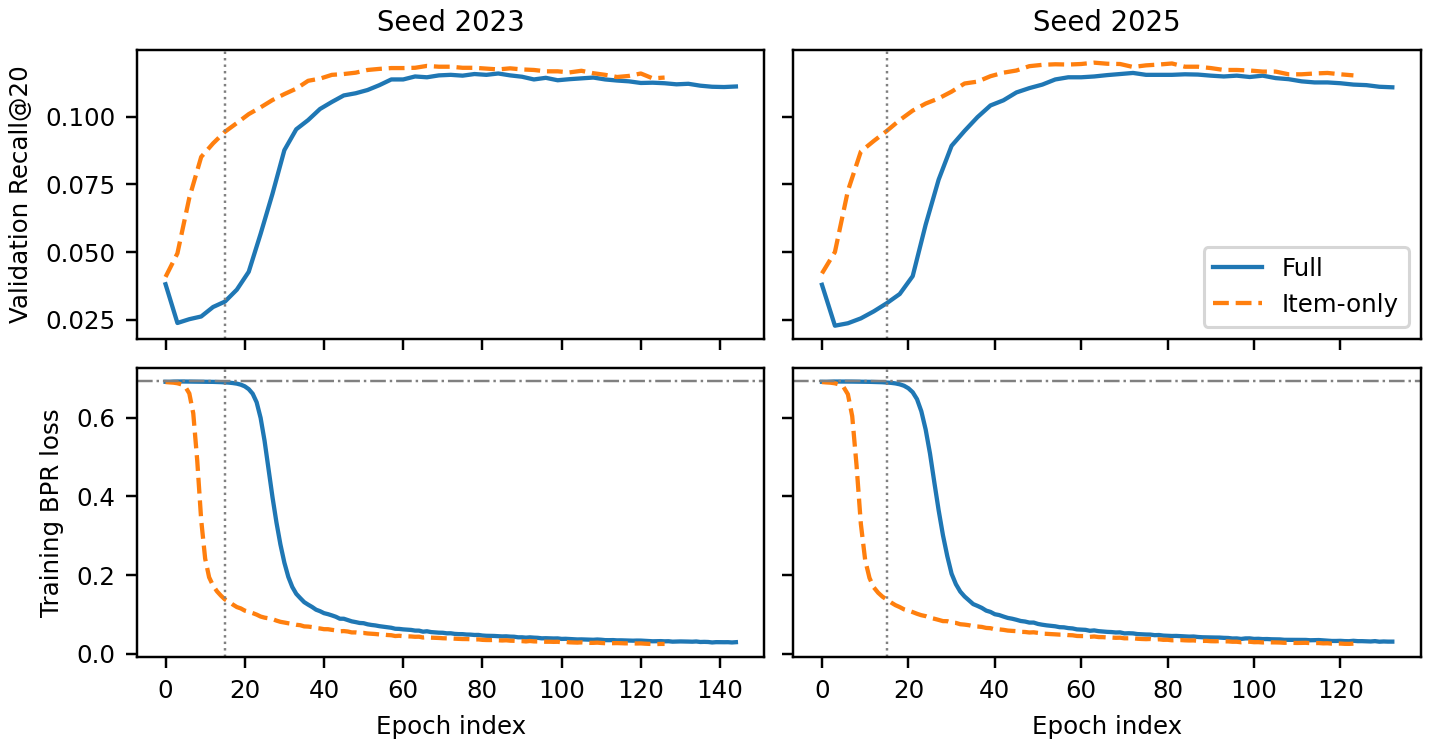
\includegraphics[width=\textwidth]{generated/patience_bpr_curves.png}
\caption{Yelp, $\alpha=0.03$, patience 20. Top: validation Recall@20. Bottom:
training BPR loss; the dash-dotted line is $\ln 2$. Dotted lines mark epoch 15,
where the five-check rule stops the full model.}
\label{fig:patience}
\end{figure}
\begin{table}[t]
\caption{Yelp $\alpha=0.03$, patience 20. Validation Recall@20 and best epoch
indices. These runs never evaluate the test set.}
\label{tab:patience}\centering\small
\begin{tabular}{rrrrr}
\toprule Seed & Full & Item-only & Full epoch & Item epoch\\\midrule
\PublicationPatienceRows
\bottomrule\end{tabular}
\end{table}
It does not really collapse; it is stopped too early. Given more patience (20
evaluations instead of five), the full model at Yelp $\alpha=0.03$ reaches
validation Recall@20 of $0.11587$ and $0.11605$ on seeds 2023 and 2025,
compared with $0.11866$ and $0.11991$ for item-only
(Table~\ref{tab:patience}). On seed 2023, the gap between the two variants
shrinks from $0.08085$ to $0.00280$. The full model still trails slightly, but
it is nowhere near a collapse.

Figure~\ref{fig:patience} shows what happens. In the full model, the BPR loss
sits at $\ln 2$ until epoch 22--23, which means the model cannot yet tell
positive items from negative ones. Meanwhile, the alignment loss falls
quickly and then levels off. Validation Recall@20 first drops below where it started at epoch 0,
and only climbs once BPR leaves this plateau. Without the user term, BPR
leaves the plateau by epoch 7. If we replay the five-evaluation stopping rule
on the logged curves, both full-model runs stop at epoch 15, right in the
middle of the plateau. With more patience, their best epochs are 84 and 72.

Two notes on this replay. The logged Recall@20 values are rounded to four
decimals, but the early drops are far larger than any rounding error. And the
replay works within each logged run, so it does not rely on MPS reruns being
bit-for-bit identical.

The curves show where training stalls, but not why. One plausible
explanation, which we have not tested, is that at this weight the user InfoNCE
term, which compares each user against all user profiles, dominates the
gradients early in training. We see no sign of a similarly early stop in the
main runs at $\alpha=0.01$: none of the 45 picked a checkpoint before epoch 24.

\subsection{RQ4: How repeatable is a single seed?}
\label{sec:resolution}
Not perfectly. Four repeats of Amazon seed 42 give test Recall@20 standard
deviations of $0.000536$ for the full model and $0.000344$ for item-only, with
ranges of $0.001090$ and $0.000810$. The full model picks epochs 66, 78, 66
and 72, while item-only picks epoch 66 every time, so scores vary even when
the chosen epoch does not.

Both standard deviations are larger than the mean Amazon difference between
item-only and full ($0.000266$), so that difference should not be read as a
precise number. Four repeats of one seed cannot tell us how much of the
variation comes from execution and how much from initialization, and the
result may not carry over to other datasets. The paired-seed intervals remain
our main measure of uncertainty.

\section{Discussion and Limitations}
\paragraph{What we found.}
Removing user-profile alignment from RLMRec-Con made no detectable difference
on Amazon (under three protocols) or Yelp, and cost about 1\% of Recall@20 and
NDCG@20 on Steam. Whether user profiles are worth the cost of generating them
therefore depends on the dataset, and has to be checked dataset by dataset.
Steam differs from the other two in two ways: it is denser (about 60 training
interactions per item, against 13 on Amazon), and it is not filtered by
rating. With only three datasets, we cannot say which of these matters.

\paragraph{A lesson for ablations.}
Before interpreting a large ablation gap, look at the training curves. On
Yelp, a patience setting that is standard for this code turned a difference
of $0.003$ into an apparent $0.081$.

\paragraph{Limitations.}
We study one backbone, three benchmarks and one fixed set of semantic inputs.
We cannot confirm how every released profile was generated, or that its
generation respected the data splits. The examples in the RLMRec repository
use GPT-3.5-turbo and text-embedding-ada-002, but examples are not generation
logs. And even though our interaction splits do not overlap, information from
the test data could still have entered the profiles when they were generated
upstream.

Deleting the user loss also lowers the total alignment weight and changes what
the shared projector learns from; a control that keeps the total alignment
weight fixed would separate these effects. Five seeds also limit what we can
detect: with this design, we have 80\% power to detect Amazon differences of
about 1.4\% of the full model's Recall@20, so smaller effects could go
unnoticed.

Even without user alignment, the model still uses each user's interaction
history, and possibly item reviews written by users, so we make no claims
about cold-start or privacy benefits. Finally, we did not contact the original
authors, so details missing from the released code were not confirmed with
them.

\paragraph{Artifact.}
The artifact contains the implementation, tests, result manifests with
checksums, per-run scores and logs, the analysis scripts that regenerate every
table and figure from the frozen results, and the manuscript sources. It
supports three checks, from cheapest to most expensive: recomputing every
reported statistic, which needs neither the data nor a GPU; checking split
disjointness, array shapes and input fingerprints once the RLMRec inputs are
installed; and retraining any configuration in the manifests into a separate
output directory. Note that identical seeds do not guarantee identical results
on MPS. Only the weight grid has a fully preserved snapshot of the source code
taken before the runs. The other runs carry source digests, which identify the
code that was used but cannot restore it. The raw datasets and semantic arrays
must be obtained from RLMRec.

\clearpage
\begin{thebibliography}{10}
\bibitem{rlmrec} Ren, X., Wei, W., Xia, L., Su, L., Cheng, S., Wang, J., Yin, D.,
Huang, C.: Representation Learning with Large Language Models for Recommendation.
In: The Web Conference (2024). \doi{10.1145/3589334.3645458}
\bibitem{lightgcn} He, X., Deng, K., Wang, X., Li, Y., Zhang, Y., Wang, M.:
LightGCN: Simplifying and Powering Graph Convolution Network for Recommendation.
In: SIGIR (2020). \doi{10.1145/3397271.3401063}
\bibitem{llmrec} Wei, W., Ren, X., Tang, J., Wang, Q., Su, L., Cheng, S., Wang, J.,
Yin, D., Huang, C.: LLMRec: Large Language Models with Graph Augmentation for
Recommendation. In: WSDM (2024). \doi{10.1145/3616855.3635853}
\bibitem{alpharec} Sheng, L., Zhang, A., Zhang, Y., Chen, Y., Wang, X., Chua, T.-S.:
Language Representations Can Be What Recommenders Need: Findings and Potentials.
In: ICLR (2025). \url{https://openreview.net/forum?id=eIJfOIMN9z}
\bibitem{dacrema} Ferrari Dacrema, M., Cremonesi, P., Jannach, D.: Are We Really
Making Much Progress? A Worrying Analysis of Recent Neural Recommendation
Approaches. In: RecSys (2019). \doi{10.1145/3298689.3347058}
\bibitem{rendle-baselines} Rendle, S., Zhang, L., Koren, Y.: On the Difficulty of
Evaluating Baselines: A Study on Recommender Systems. arXiv:1905.01395 (2019)
\bibitem{bouthillier} Bouthillier, X., Delaunay, P., Bronzi, M., Trofimov, A.,
Nichyporuk, B., Szeto, J., Sepah, N., Raff, E., Madan, K., Voleti, V., Ebrahimi
Kahou, S., Michalski, V., Serdyuk, D., Arbel, T., Pal, C., Varoquaux, G.,
Vincent, P.: Accounting for Variance in Machine Learning Benchmarks. In: MLSys
(2021)
\bibitem{bpr} Rendle, S., Freudenthaler, C., Gantner, Z., Schmidt-Thieme, L.: BPR:
Bayesian Personalized Ranking from Implicit Feedback. In: UAI (2009)
\bibitem{infonce} van den Oord, A., Li, Y., Vinyals, O.: Representation Learning
with Contrastive Predictive Coding. arXiv:1807.03748 (2018)
\bibitem{freedom} Zhou, X., Shen, Z.: A Tale of Two Graphs: Freezing and Denoising
Graph Structures for Multimodal Recommendation. In: ACM Multimedia (2023).
\doi{10.1145/3581783.3611943}
\bibitem{holm} Holm, S.: A Simple Sequentially Rejective Multiple Test Procedure.
Scandinavian Journal of Statistics \textbf{6}(2), 65--70 (1979)
\end{thebibliography}
\end{document}